\section{Results}
To demonstrate the potency of our approach we have solved the TSP problem for
multiple data sets. We compare the optimal results to the results found using
the combination of renormalization and TSA. To analyze the quality of the
proposed technique the state of the system while seeking the solution for two
different data sets is compared.

\subsection{Overall Results}
The shortest route for multiple problems was computed to demonstrate the
improvement allowed by the TSA process. The problems used vary in
the number of cities. To find an optimal result the only parameter which was
changed is the beginning temperature of the TSA process. This
is necessary to prevent very high acceptance rates (see equation
\ref{eq:accept}) and provoke large entropy changes (see equation
\ref{eq:entropy}). In general the initial temperature is higher for data sets
with a large amount of cities than for a low amount of cities.

In figure \ref{fig:results}~an overview is given of the results found. The
dark dots represent the optimal solution found at the end of the TSA process.
The circles designate the solution found if TSA would not be used. The
triangles denote the worst solution found during the TSA process. It is clear
from the picture that seeking an optimal rotation angle leads to better
approximations of the shortest route. Yet, as we shall see in the next section
TSA also partly undoes the computational benefit obtained by using renormalization.

\ctable[caption={The results found compared to the shortest route for various
	numbers of cities},
		 label={fig:results},
		 figure]{c}{\tnote[]{This figure shows the quality of the results found
		 using the renormalization process combined with the TSA.\\
		 The circles show the approximation error when not using TSA. The dark
		 dots show the optimal value found using TSA. The triangles denote the
		 worse solution found during the TSA process.\\
		 It can be concluded that using TSA improves the results
		 considerably.}}{\FL 
		 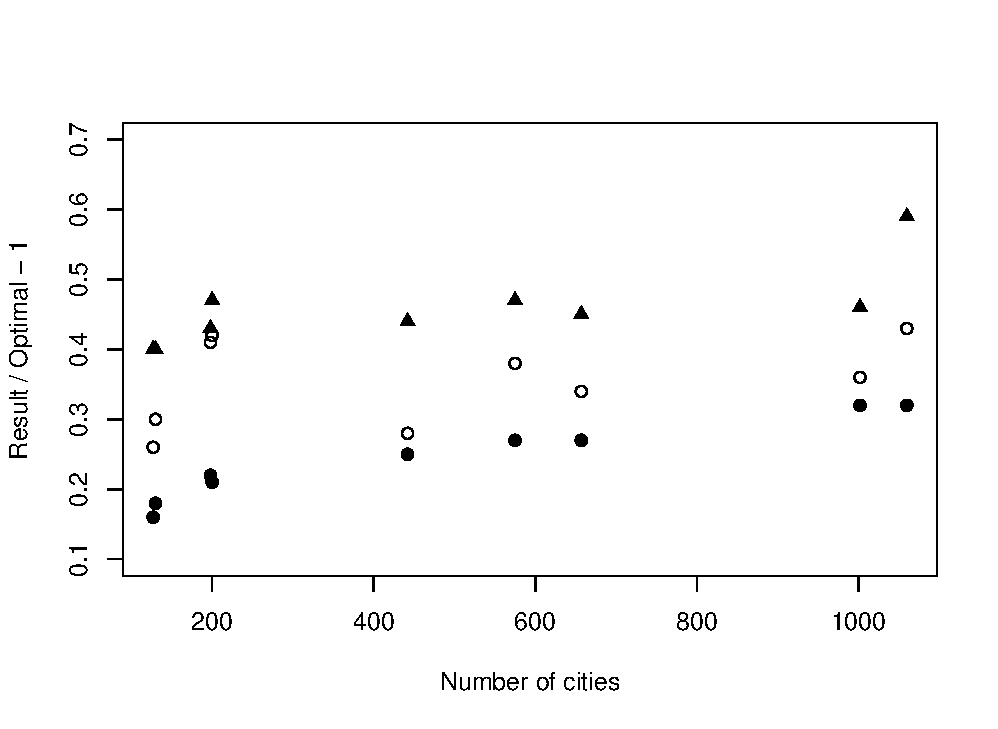
\includegraphics[width=8cm]{fig/results}
		 \LL}

\subsection{Two data sets compared}
To show that the TSA process increases the computing time considerably we
analyze the dynamics of the system while solving two data sets. The first data
set contains 198 cities which are concentrated in a few clusters, see Fig.
\ref{fig:d198}. In contrast, the second data set which contains 575 cities is
much more uniformly distributed, see Fig. \ref{fig:rat575}.

The dynamics of the TSA process while solving both problems are showed in Fig.
\ref{fig:res198}~for 198 cities and in Fig. \ref{fig:res575}~for 575 cities.
In both cases the convergence of the temperature to the end temperature takes
very long. While in the case of 198 cities the reduction of the temperature
also leads to a lower energy, this is not case for 575 cities. Analogue to the
annealing process in metallurgy, it is possible that the temperature
diminishes and that the system maintains a high energy, resulting in a
non-optimal system. This is clearly the case when solving the second problem set.

The delayed reduction of the change of the rotation angle when the temperature
of the system diminishes is attributed to the value of the initial
temperature. In the case of 198 cities the initial temperature is set to 1000.
For 575 cities the temperature is set to 5000. For the first problem this
barrier is crossed at time 100, for the second this is around time 5600.  It
is clear that after these times rotation angle change reduces.

The reason why TSA is used is to seek for several optima and then to select
the global optimum found and then fine tune the rotation angle to improve the
optimum. Yet the auto-adjusting cooling schedule does not always lead to this
behaviour. For the first data set, the rotation angle at which the shortest
route is found is 0.9258 $\pi$ radian, the rotation angle found at the lowest
temperature is identical. However for the 575 cities problem system is cool at
a rotation angle of 0.0112 $\pi$ radian. Which is not close to the optimal rotation
angle of 2.3126 $\pi$ radian. This latter observation supports our claim that the
second system is not in an optimal state.

In the case of 575 cities the shortest route is quickly found. This is
attributed to the perturbation function. Because of the large scale of the
graphs in Fig. \ref{fig:rat575} it is not immediately clear that at the
beginning the perturbation function allows to visit many different states.
Thereby enabling the system to find a shortest route. For the 198 cities
problem it takes longer to find the optimum. Only once the system is much
cooler the solution is found by fine-tuning the rotation angle.

Although the TSA permits to find a optimal solution the computational costs
are considerably increased. Considering the 575 cities problem more than 13000
iterations are necessary to cool the system to an appropriate temperature. For
the 198 cities problem 2500 iterations are necessary. Other problem sets
we considered needed 13000 iterations for 1002 cities and 1100 iterations for
200 cities.

\subsection{Conclusion}
Improving the classical renormalization algorithm using a TSA process improves
the accuracy of the result. However the computational costs increase considerably.
Most of the time is consumed towards the end of the convergence of the
temperature. This could be reduced by using another cooling schedule then the 
auto-adjusting schedule used by the TSA.

\ctable[caption={The location of the cities in the 198 cities problem},
		 label={fig:d198},
		 figure]{c}{\tnote[]{This figure shows how 198 cities are distributed
		 over the entire pane. The interesting feature of this problem is that
		 the cities are concentrated in clusters.}}{\FL
		 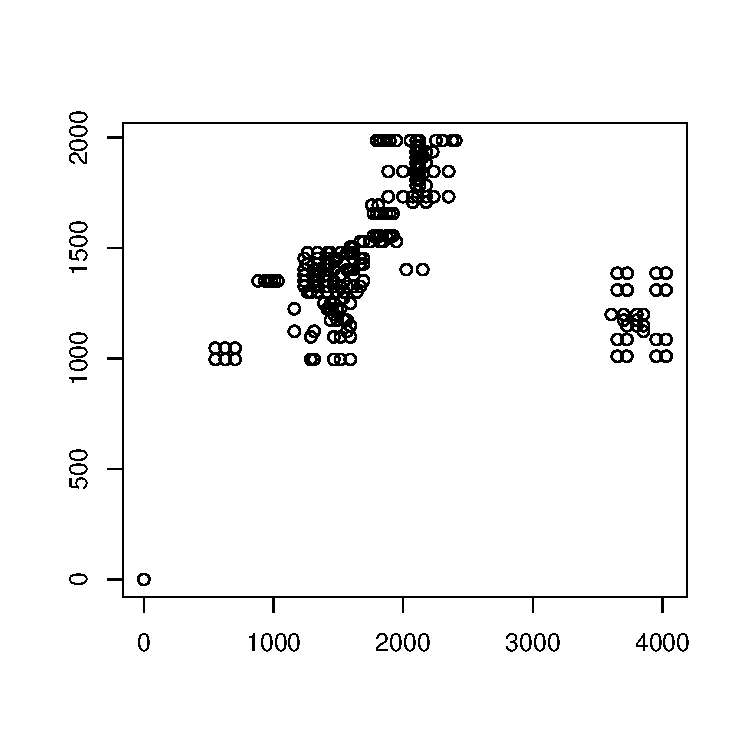
\includegraphics[width=7cm]{fig/d198cities}
		 \LL}

\ctable[caption={The location of the cities in the 575 cities problem},
		 label={fig:rat575},
		 figure]{c}{\tnote[]{This figure shows how 575 cities are distributed
		 over the entire pane. An aspect of this data set is that the cities are
		 distributed almost uniformly over the pane.}}{\FL
		 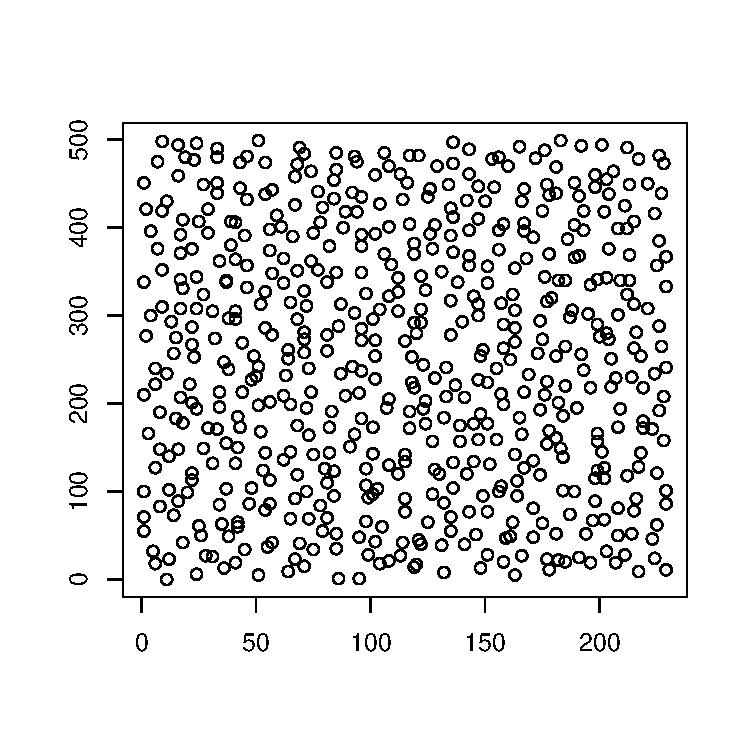
\includegraphics[width=7cm]{fig/rat575cities}
		 \LL}


\ctable[caption={Properties of the system when seeking the shortest route
		connecting 198 cities},
		label={fig:res198},
		figure,
		star]{c}{\tnote[]{These graphs show the state of the TSA process which
		searches the optimal rotation angle for the cities displayed in figure
		\ref{fig:d198}. The first figure shows the amount of energy present in
		the system. The second displays the temperature. The third the found
		rotation angle. The last shows the shortest route found until a point in
		time.\\
		Because the energy in the system approaches zero at the end of the
		process the system is in equilibrium. The equilibrium is found at an
		angle of 0.9258 $\pi$ radian.}}{\FL
		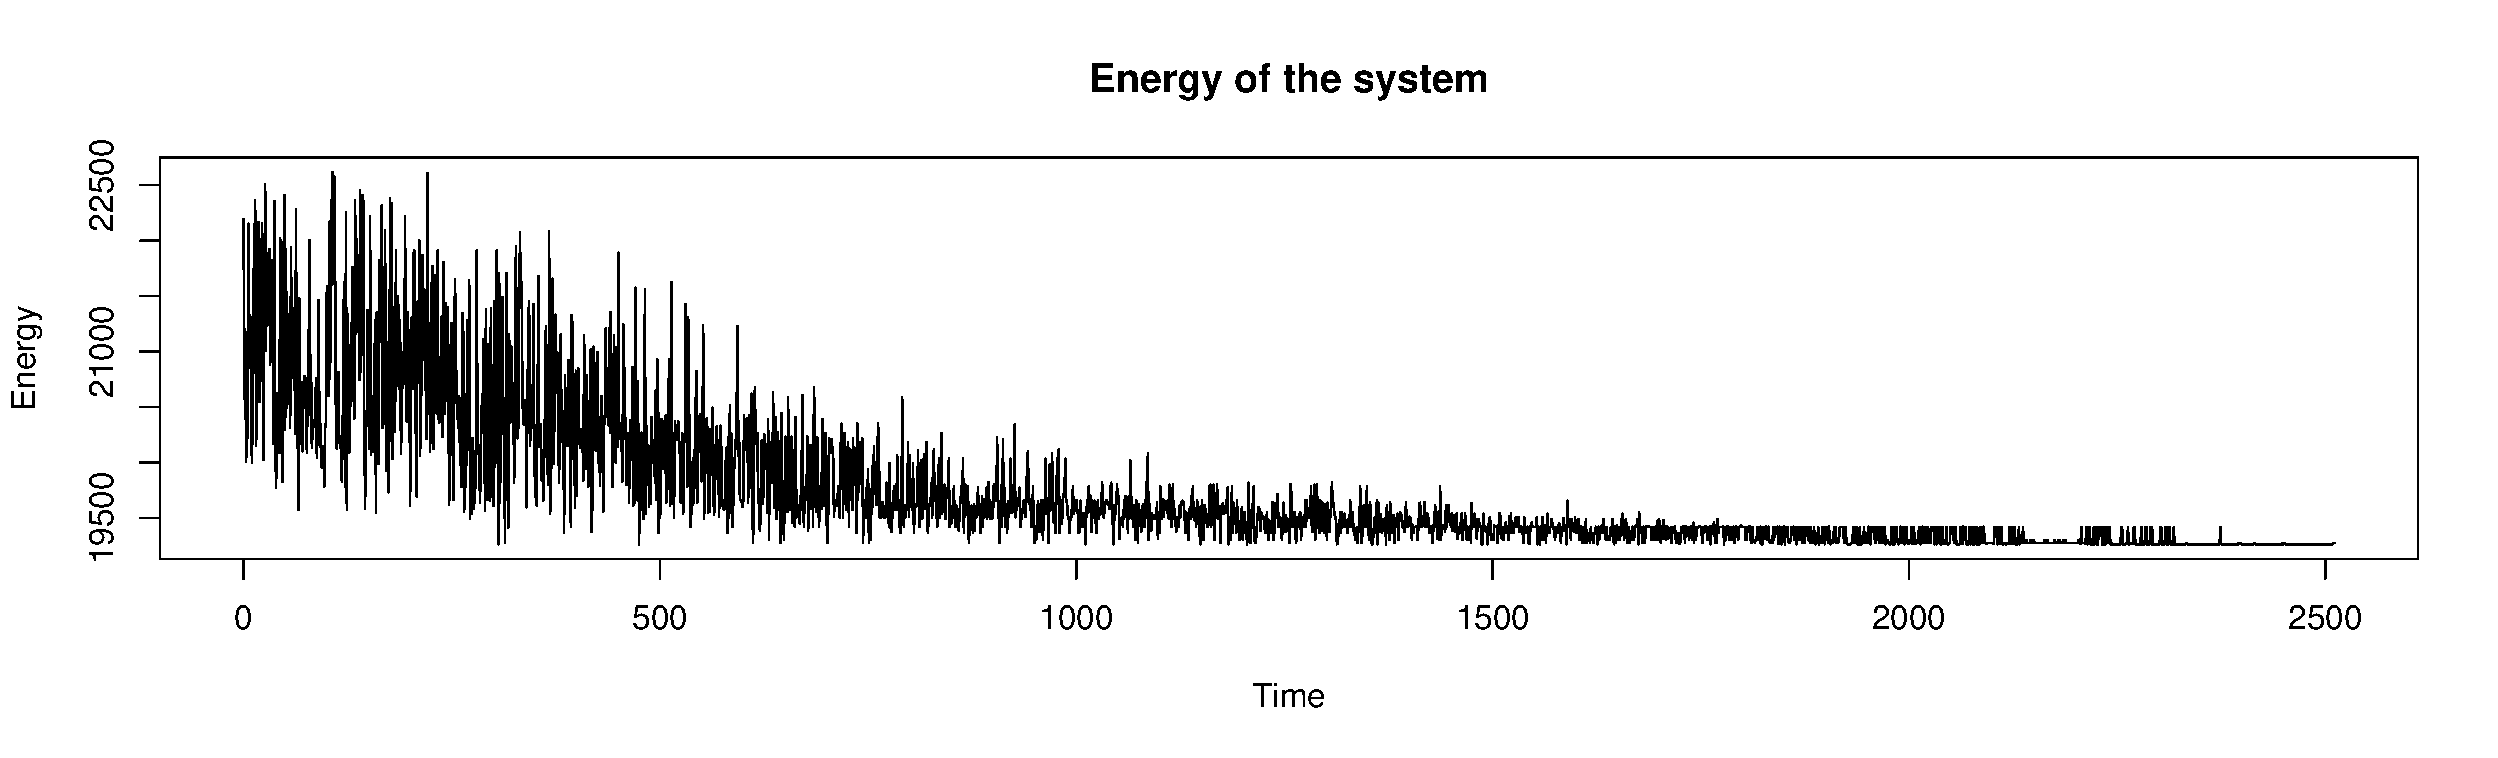
\includegraphics[width=15cm]{fig/d198energy}\NN
		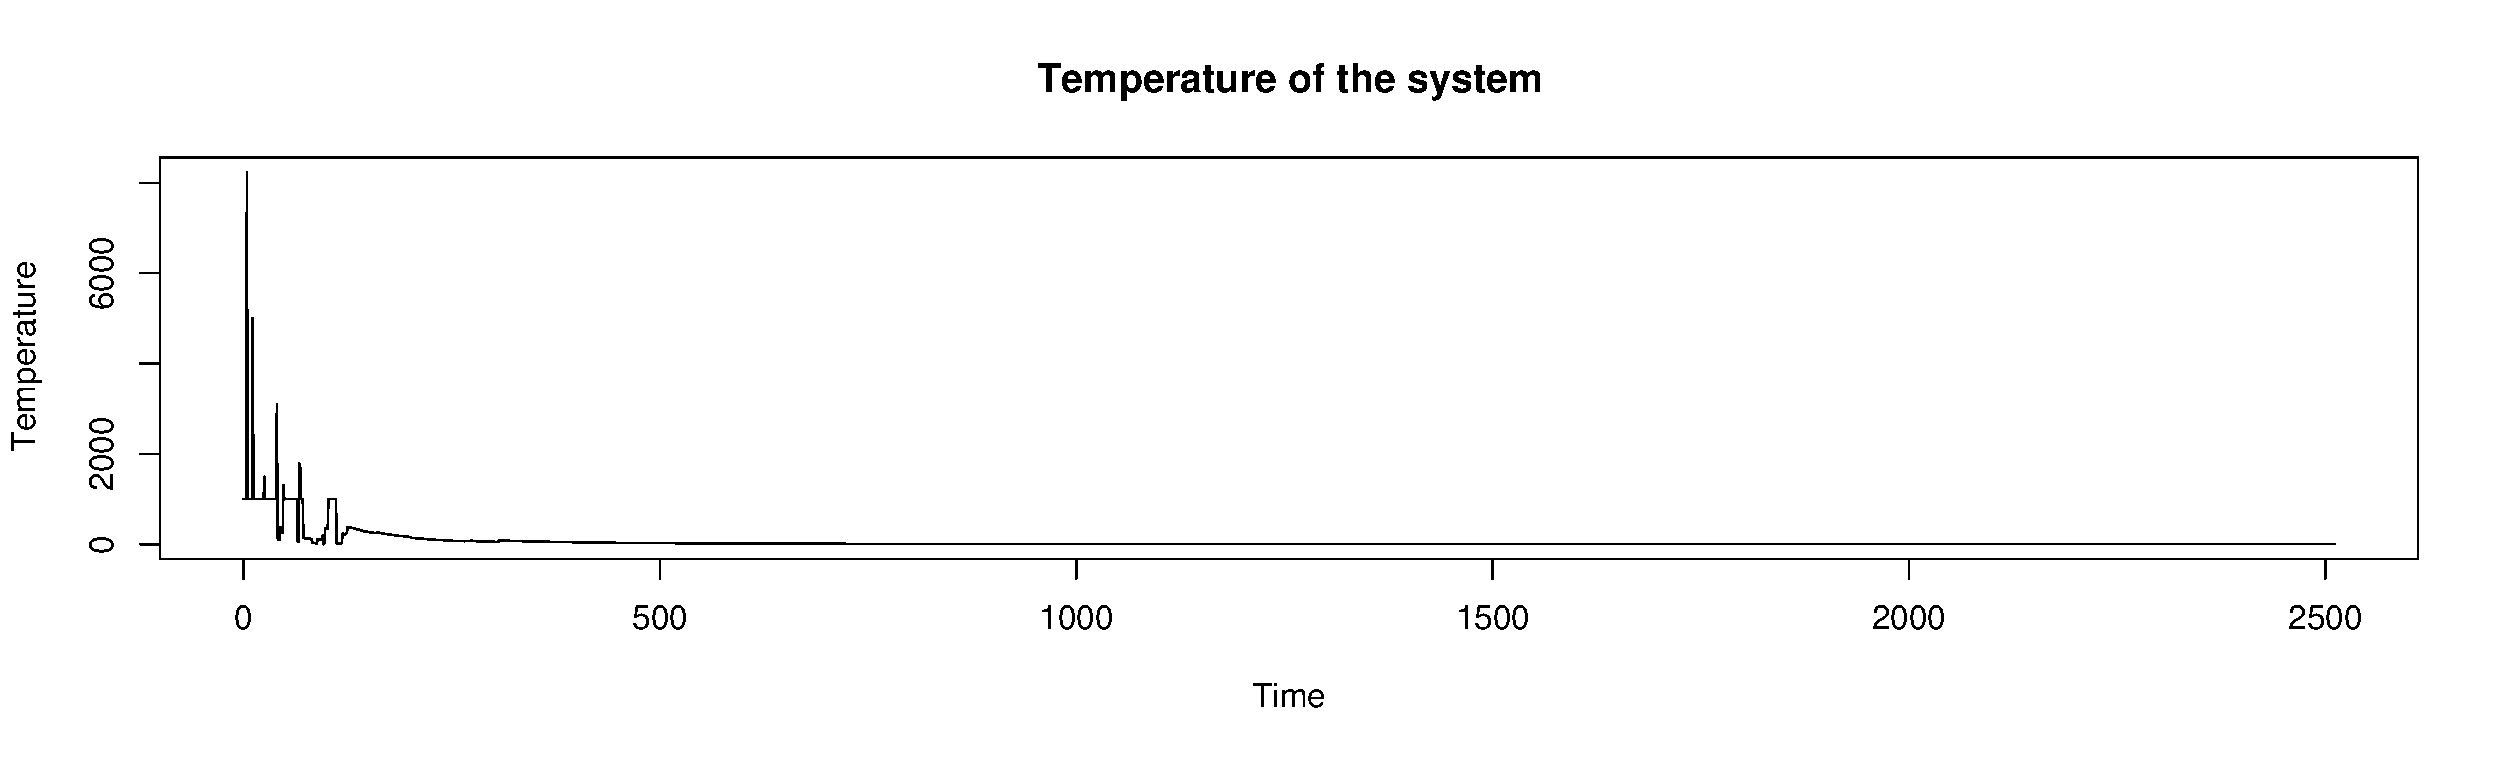
\includegraphics[width=15cm]{fig/d198temp}\NN
		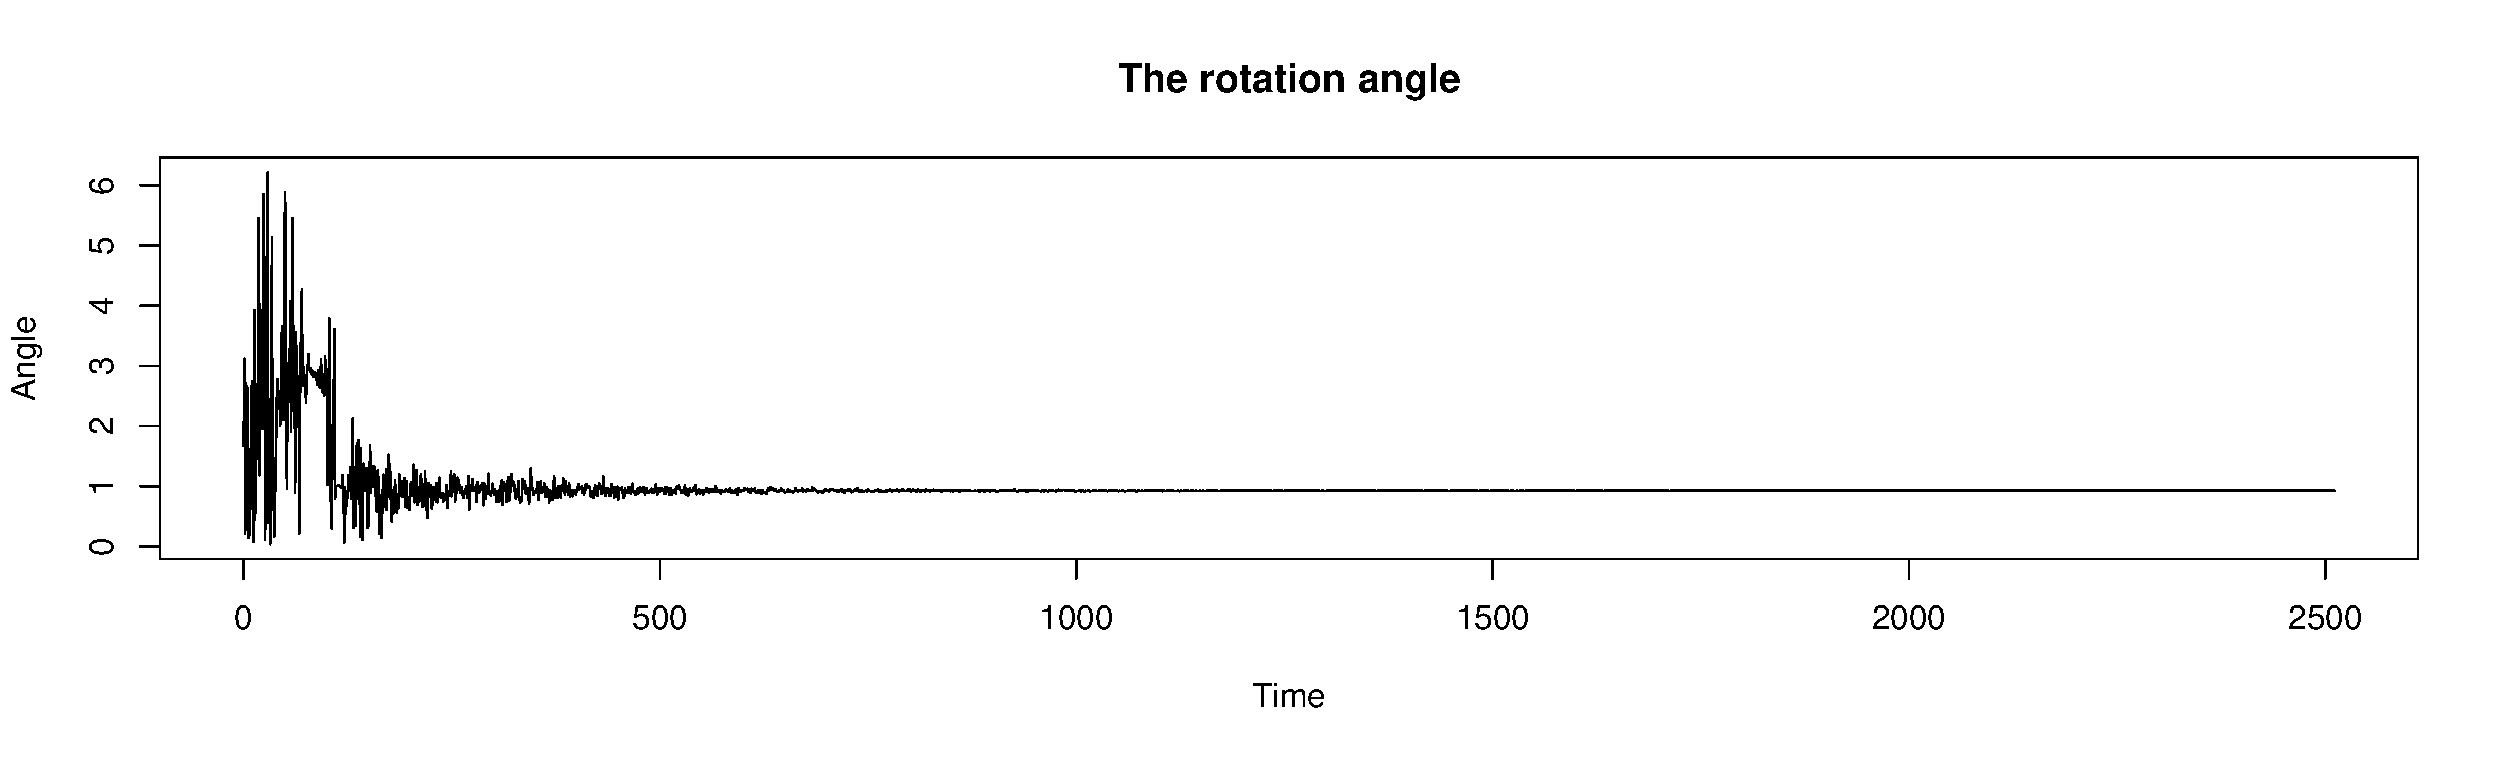
\includegraphics[width=15cm]{fig/d198rotation}\NN
		\includegraphics[width=15cm]{fig/d198shortest}\LL}

\ctable[caption={Properties of the system when seeking the shortest route
		connecting 575 cities},
		label={fig:res575},
		figure,
		star]{c}{\tnote[]{These graphs show the state of the TSA process which
		searches the optimal rotation angle for the cities displayed in figure
		\ref{fig:d198}. The first figure shows the amount of energy present in
		the system. The second displays the temperature. The third the found
		rotation angle. The last shows the shortest route found until a point in
		time.\\
		In the upper figure can be seen that the TSA is unable to find a state
		where the temperature and the energy are low. This undesirable state
		leads to a rotation angle of 0.0112 $\pi$ radian which defers
		considerably from the optimal result 2.3126 $\pi$ radian.
		}}{\FL
		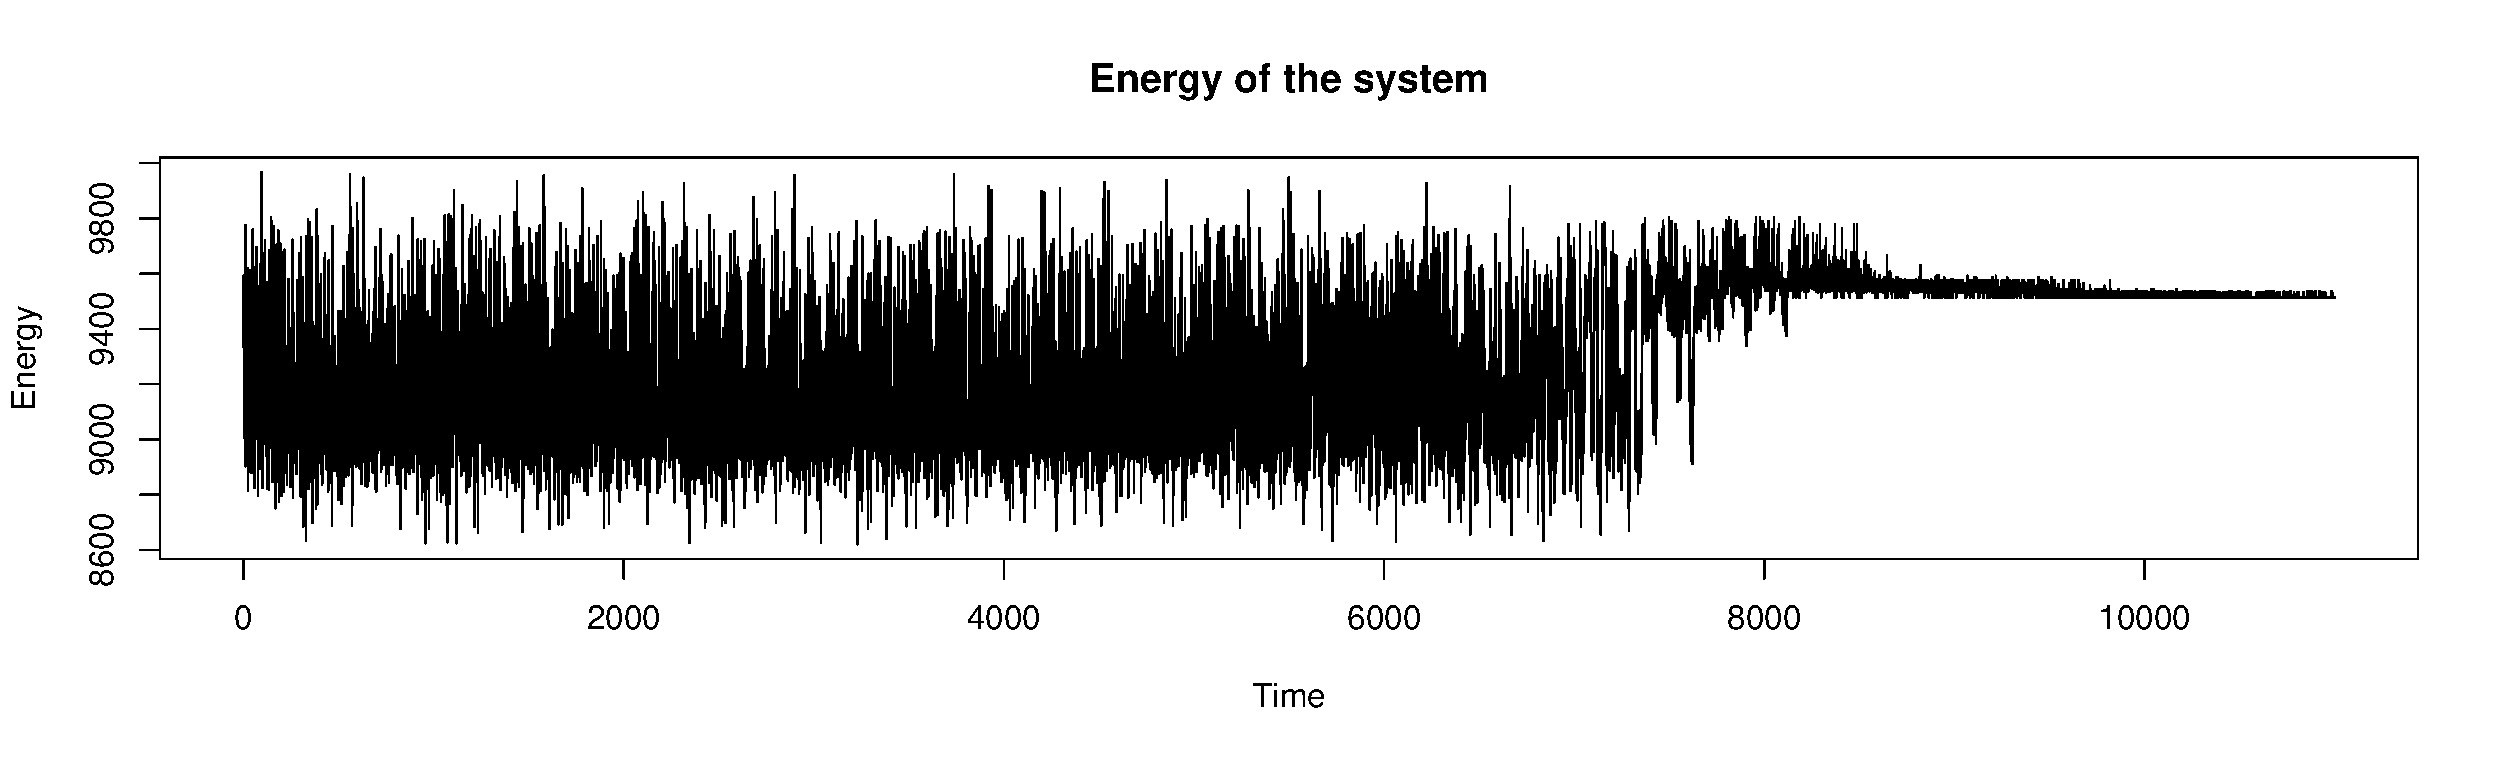
\includegraphics[width=15cm]{fig/rat575energy}\NN
		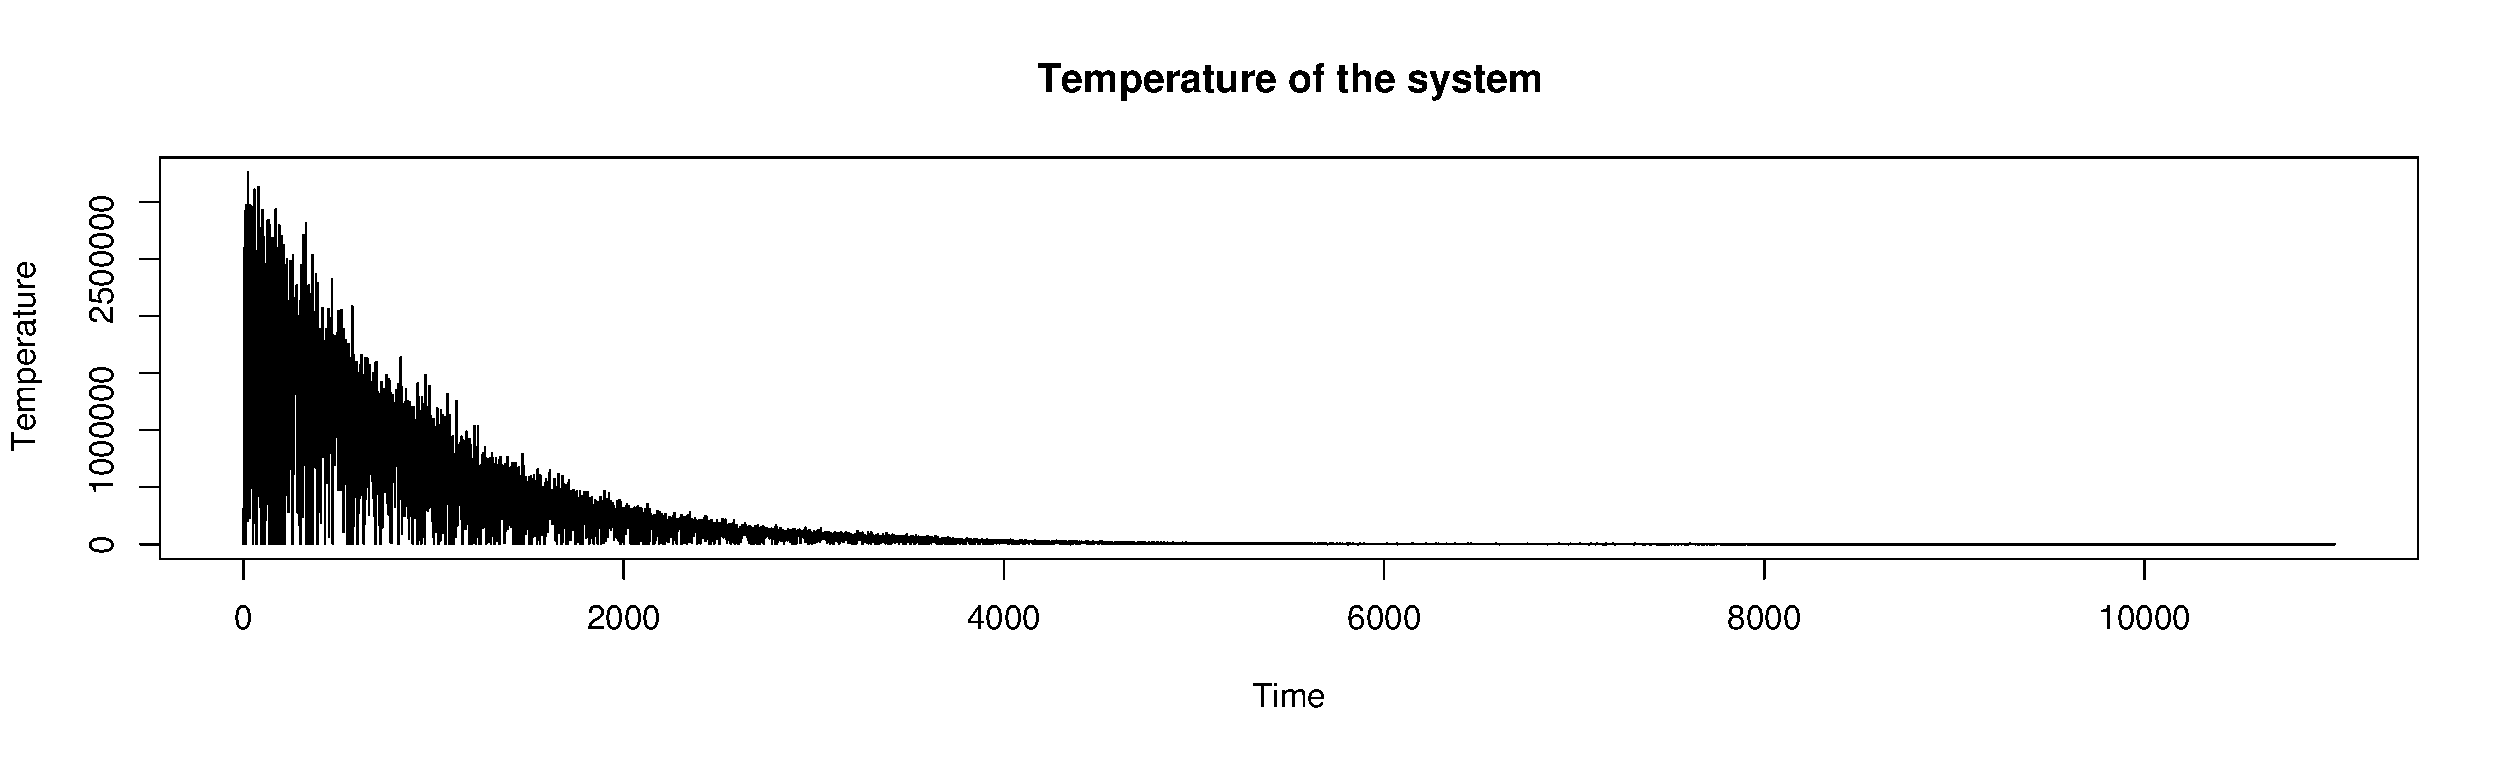
\includegraphics[width=15cm]{fig/rat575temp}\NN
		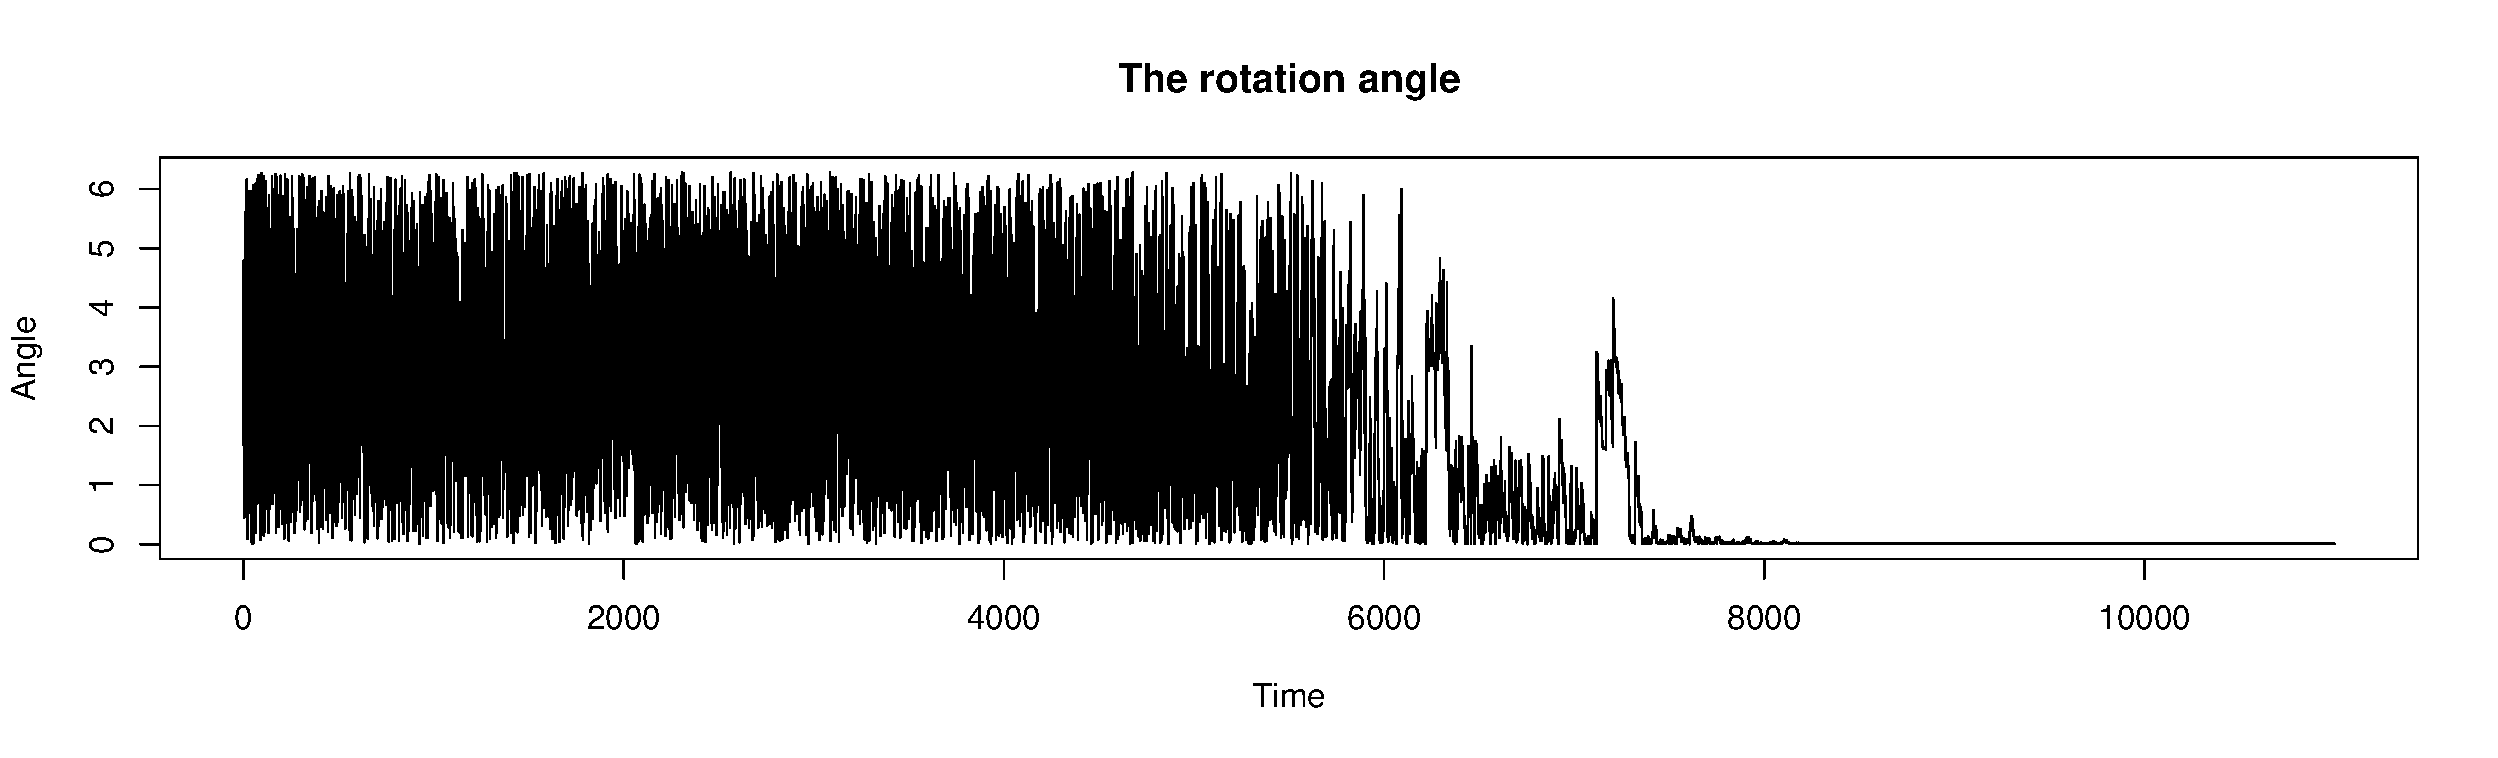
\includegraphics[width=15cm]{fig/rat575rotation}\NN
		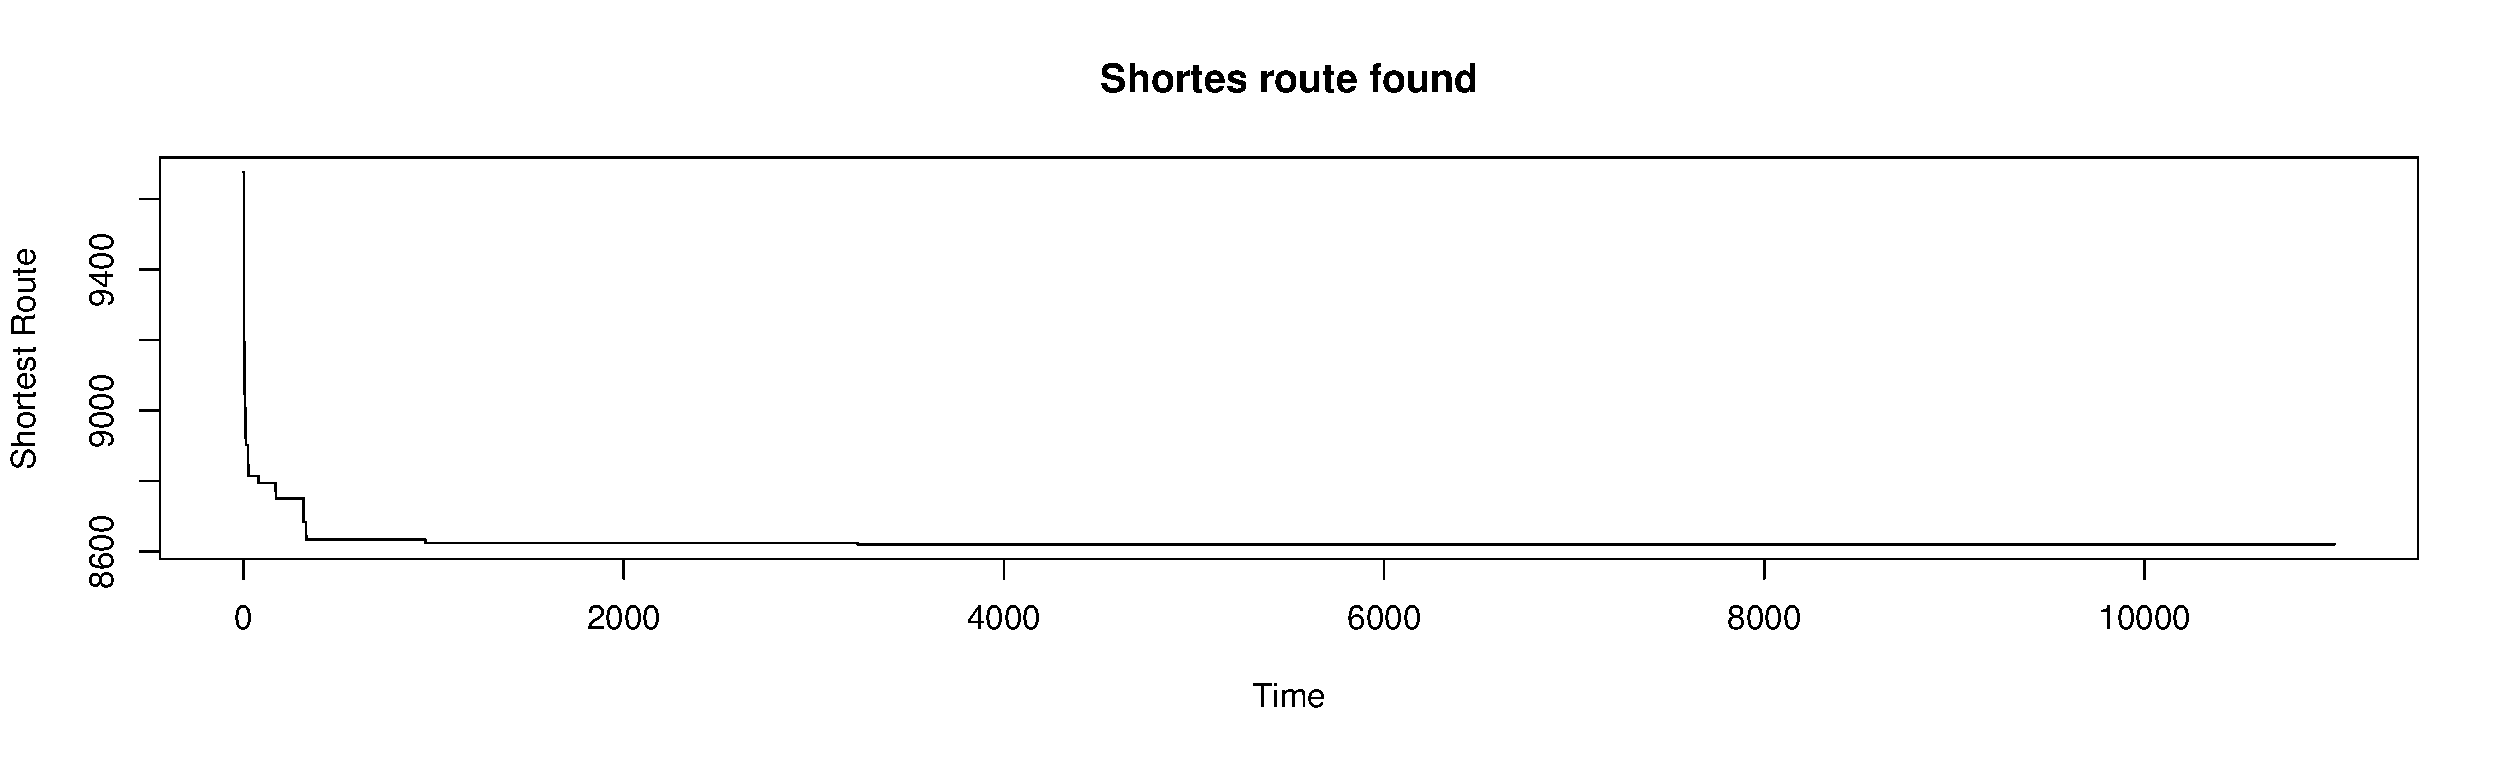
\includegraphics[width=15cm]{fig/rat575shortest}\LL}

% vim:ft=tex:spell spelllang=en:autoindent

